\chapter{Considerações Gerais}
\label{cap:02}


\section{Dogma Central da Biologia Molecular}

O dogma central da biologia molecular descreve o fluxo da informação genética nos sistemas biológicos. Formulado por \citeauthorandyear{Crick1958} e reapresentado por \citeauthorandyear{Crick1970}, estabelece que a informação de sequência pode ser transferida de ácido nucleico para ácido nucleico ou de ácido nucleico para proteína, mas não de proteína para proteína nem de proteína para ácido nucleico \cite{Crick1970}. Esse postulado se apoia na hipótese da sequência, segundo a qual a ordem das bases de um segmento de ácido nucleico determina a ordem dos aminoácidos de uma proteína \cite{Crick1958}.

O fluxo ocorre por três processos: replicação, transcrição e tradução. A replicação é a duplicação do ácido desoxirribonucleico (DNA), possível porque a dupla hélice é formada por fitas complementares \cite{WatsonCrick1953}. É semiconservativa, pois cada molécula-filha conserva uma fita parental \cite{MeselsonStahl1958}. A transcrição é a síntese de ácido ribonucleico (RNA) complementar a um segmento de DNA, e os genes que codificam proteínas originam RNAs mensageiros (mRNA) \cite{Nelson2014}. Em eucariotos, o transcrito primário é processado por adição de \textit{cap}, remoção de íntrons (\textit{splicing}) e poliadenilação \cite{Alberts2017}.

A tradução é a síntese de um polipeptídeo a partir do mRNA, realizada nos ribossomos com o auxílio de RNAs transportadores (tRNA), que reconhecem os códons por pareamento de bases \cite{Nelson2014}. O código genético é lido em trincas de nucleotídeos \cite{Crick1961}, e sua correspondência com os aminoácidos foi elucidada por \citeauthorandyear{Nirenberg1961}. Dos 64 códons possíveis, 61 especificam aminoácidos e três sinalizam o término da tradução; como há 20 aminoácidos, o código é degenerado \cite{Nelson2014}.

Esses processos correspondem às transferências gerais do dogma: DNA $\rightarrow$ DNA, DNA $\rightarrow$ RNA e RNA $\rightarrow$ proteína \cite{Crick1970}. O dogma admite ainda transferências especiais, como RNA $\rightarrow$ RNA, RNA $\rightarrow$ DNA e DNA $\rightarrow$ proteína \cite{Crick1970}; a transcrição reversa em retrovírus é um exemplo de RNA $\rightarrow$ DNA \cite{Temin1970, Baltimore1970}. O que o dogma exclui são as transferências a partir de proteínas \cite{Crick1970}. Os príons, agentes infecciosos de natureza proteica \cite{Prusiner1982}, não contradizem esse postulado, pois se propagam por alteração conformacional de uma proteína do hospedeiro, sem alterar sua sequência \cite{Alberts2017}.

\section{DNA, RNA e Proteínas}

\subsection{Ácidos Nucleicos}

Os ácidos nucleicos são polímeros lineares de nucleotídeos, cada um formado por uma base nitrogenada, uma pentose e um grupo fosfato \cite{Nelson2014}. Os nucleotídeos se unem por ligações fosfodiéster entre o carbono $3'$ de uma pentose e o carbono $5'$ da seguinte, o que confere polaridade $5' \rightarrow 3'$ à cadeia \cite{Nelson2014}. As bases são purinas, adenina (A) e guanina (G), ou pirimidinas, citosina (C), timina (T) e uracila (U) \cite{Nelson2014}.

O DNA contém desoxirribose e as bases A, G, C e T, enquanto o RNA contém ribose e substitui a timina pela uracila \cite{Nelson2014}. As regularidades descritas por \citeauthorandyear{Chargaff1950}, segundo as quais as quantidades de A e T são iguais, assim como as de G e C, foram explicadas pelo modelo de dupla hélice de \citeauthorandyear{WatsonCrick1953}, construído com apoio em dados de difração de raios X \cite{Franklin1953}, no qual duas fitas antiparalelas se pareiam por ligações de hidrogênio, A com T (duas ligações) e G com C (três ligações) \cite{Nelson2014}. Um gene é um segmento de DNA com a informação para um produto funcional, proteína ou RNA, e o genoma é o conjunto de toda a informação genética do organismo \cite{Alberts2017}.

O RNA ocorre, em geral, como fita simples \cite{Nelson2014}. Além do mRNA, que veicula a informação para a síntese proteica, destacam-se o tRNA e o RNA ribossômico (rRNA), componente estrutural e catalítico do ribossomo \cite{Alberts2017}.

\subsection{Aminoácidos e Proteínas}

As proteínas são polímeros de aminoácidos com funções estruturais, catalíticas, de transporte e de defesa, entre outras \cite{Nelson2014}. Os 20 aminoácidos usuais compartilham um carbono $\alpha$ ligado a um grupo amino, um grupo carboxil e um hidrogênio, e diferem pelo grupo R, ou cadeia lateral \cite{Nelson2014}. Conforme a polaridade e a carga do grupo R, são classificados em cinco grupos, apresentados na Tabela~\ref{tab:aminoacidos} com os códigos de três letras e de uma letra, esta última usada para representar sequências.

\FloatBarrier
\begin{table}[!htbp]
	\centering
	\SingleSpacing\small
	\caption{Classificação dos 20 aminoácidos usuais segundo as propriedades do grupo R}
	\begin{tabularx}{\textwidth}{@{}lX@{}}
		\toprule
		\textbf{Grupo} & \textbf{Aminoácidos (três letras, uma letra)} \\
		\midrule
		Apolares alifáticos      & Gly (G), Ala (A), Pro (P), Val (V), Leu (L), Ile (I), Met (M) \\
		Aromáticos               & Phe (F), Tyr (Y), Trp (W) \\
		Polares sem carga        & Ser (S), Thr (T), Cys (C), Asn (N), Gln (Q) \\
		Carregados positivamente & Lys (K), Arg (R), His (H) \\
		Carregados negativamente & Asp (D), Glu (E) \\
		\bottomrule
	\end{tabularx}
	\par\vspace{0.2cm}
	\textbf{Fonte:} Adaptada de \citeonline{Nelson2014}
	\label{tab:aminoacidos}
\end{table}

Os aminoácidos se unem por ligações peptídicas, formadas pela condensação do grupo carboxil de um com o grupo amino do seguinte, com liberação de água \cite{Nelson2014}. A cadeia resultante, o polipeptídeo, tem sentido da extremidade amino-terminal (N-terminal) à carboxi-terminal (C-terminal), e cada aminoácido incorporado é denominado resíduo \cite{Nelson2014}.

A organização das proteínas é descrita em quatro níveis \cite{Nelson2014}. A estrutura primária é a sequência linear de resíduos. A secundária corresponde a padrões locais regulares do esqueleto polipeptídico, estabilizados por ligações de hidrogênio, como a $\alpha$-hélice \cite{Pauling1951} e a folha $\beta$. A terciária é o arranjo tridimensional de um polipeptídeo, estabilizado por interações entre as cadeias laterais. A quaternária descreve o arranjo das subunidades em proteínas com mais de uma cadeia. Muitas proteínas possuem ainda domínios, regiões que se dobram de forma relativamente independente e se associam a funções específicas \cite{Alberts2017}. \citeauthorandyear{Anfinsen1973} demonstrou que a sequência primária contém a informação necessária ao dobramento.

\subsection{Enzimas e Relação entre Sequência, Estrutura e Função}

As enzimas são catalisadores biológicos, em sua maioria proteínas, que aceleram reações por reduzirem a energia de ativação \cite{Nelson2014}. A catálise ocorre no sítio ativo, formado por resíduos que ligam o substrato e participam da reação; como o sítio resulta do dobramento, resíduos distantes na estrutura primária podem estar próximos no espaço \cite{Nelson2014}. As enzimas são classificadas pela Comissão de Enzimas (\textit{Enzyme Commission}, EC) conforme a reação catalisada; as transferases, que transferem grupos funcionais entre moléculas, incluem as metiltransferases, que transferem grupos metil, em geral a partir da S-adenosilmetionina \cite{Nelson2014}.

Como a sequência determina a estrutura e esta determina a função, a sequência de aminoácidos é a base para inferir a função de uma proteína \cite{Nelson2014}. Na evolução, a estrutura tridimensional é mais conservada do que a sequência, de modo que proteínas de sequências divergentes podem manter dobramentos semelhantes \cite{Chothia1986}. Resíduos essenciais à estrutura ou à atividade, como os do sítio ativo, tendem a ser conservados, e substituições entre aminoácidos de propriedades semelhantes (Tabela~\ref{tab:aminoacidos}) são mais toleradas \cite{Nelson2014}. Essa conservação diferencial permite quantificar o parentesco entre proteínas pela comparação de suas sequências.


\section{Algoritmos de Alinhamento de Sequências}
o quanto baste


\section{Café}
o quanto baste


\section{Título}
essa seção você vai usar para explicar mais conceitos importantes para o seu trabalho.
troque o título.
você tem liberdade para adicionar, remover ou trocar as seções de ordem.



Texto das considerações gerais, dividido em subseções.

Este é um exemplo de como usar figuras. Referência cruzada: Figura~\ref{fig:exemplo}

\FloatBarrier
\begin{figure}[!htbp]
	\centering
	\caption{Exemplo de figura}
	%scale redimensiona a figura.
	%1.5 = 150% do tamanho original
	%1 = 100% do tamanho original
	%0.20 = 20% do tamanho original
	
\includegraphics[scale=0.4]{imagens/exemploFigura}
	\\\textbf{Fonte:} Elaborada pelo autor
	\label{fig:exemplo}
\end{figure}
\FloatBarrier


Este é um exemplo de como usar tabelas. Referência cruzada: Tabela~\ref{tab:exemplo}

\FloatBarrier
\begin{table}[!htbp]
	\centering
	\caption{Exemplo de tabela de 2 colunas}
	\begin{tabular}{ c | c }
		\hline
		\textbf{Coluna 1} & \textbf{Coluna 2} \\ \hline
		Dado 1a           & Dado 2a           \\ \hline
		Dado 1b           & Dado 2b           \\ \hline
		Dado 1c           & Dado 2c           \\ \hline
		Dado 1d           & Dado 2d           \\ \hline
	\end{tabular}
	\\ \vspace{0.2cm}
	\textbf{Fonte:} Elaborada pelo autor
	\label{tab:exemplo}
\end{table}
\FloatBarrier


Este é um exemplo de como usar quadros. Referência cruzada: Quadro~\ref{qua:exemplo}

\FloatBarrier
\begin{quadro}[!htbp]
	\centering
	\caption{Exemplo de quadro}
	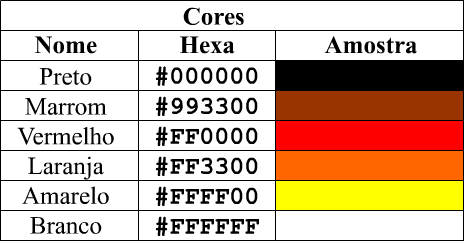
\includegraphics[scale=.7]{imagens/exemploQuadro}
	\\\textbf{Fonte:} Elaborada pelo autor
	\label{qua:exemplo}
\end{quadro}
\FloatBarrier


Este é um exemplo de como usar equações. Referência cruzada: Equação~\ref{eq:exemplo}

\begin{equation}
\sum_{i=1}^{n} i = \frac{n(n+1)}{2}
\label{eq:exemplo}
\end{equation}


Exemplo de inserção de lista de código fonte:

\lstinputlisting[language=Java]{fontes/ClasseExemplo.java} 



Este é um exemplo de como inserir texto sem formatação (ambiente verbatim):

\begin{verbatim}
Texto sem formatação, como espaçamento igual.
\end{verbatim}


Exemplo de lista de itens:

\begin{itemize}
	\item \textbf{Item 1:} texto...;
	\item \textbf{Item 2:} texto...;
	\begin{itemize}
		\item \textbf{Subitem:} texto...;
		\item \textbf{Subitem:} texto...;
		\item \textbf{Subitem:} texto...;
	\end{itemize}
	\item \textbf{Item 3:} texto...;
	\item \textbf{Item n:} texto....
\end{itemize}


Exemplo de lista numerada:

\begin{enumerate}
	\item \textbf{Item:} texto...;
	\item \textbf{Item:} texto...;
	\begin{enumerate}
		\item \textbf{Subitem:} texto...;
		\item \textbf{Subitem:} texto...;
		\item \textbf{Subitem:} texto...;
	\end{enumerate}
	\item \textbf{Item:} texto...;
	\item \textbf{Item:} texto....
\end{enumerate}


Exemplos de comandos para texto e referências:

\begin{itemize}
	\item Para iniciar um novo parágrafo, basta deixar uma linha em branco no código fonte;
	\item Não force o compilador a pular mais de uma linha, pois terá influência negativa na composição do documento;
	\item Sempre deixe o \LaTeX\ realizar a formatação de parágrafos e posicionamento de elementos;
	\item Utilização de aspas simples (abertura \verb|`|, fechamento \verb|'|): `Texto entre aspas simples';
	\item Utilização de aspas duplas (abertura \verb|``|, fechamento \verb|''|): ``Texto entre aspas duplas'';
	\item Negrito (comando \verb|\textbf|): \textbf{texto em negrito};
	\item Itálico (comando \verb|\textit|): \textit{texto em itálico};
	\item Sublinhado (comando \verb|\underline|): \underline{texto sublinhado};
	\item Negrito e itálico (usar comandos juntos): \textbf{\textit{texto em negrito e itálico}};
	\item Alterar cor do texto (comando \verb|\textcolor{cor}{texto}|):
	\begin{itemize}
		\item Exemplo \verb|\textcolor{red}{texto}|: \textcolor{red}{texto vermelho};
		\item Exemplo \verb|\textcolor[RGB]{255, 102, 0}|: \textcolor[RGB]{255, 102, 0}{texto laranja};
		\item Exemplo \verb|\textcolor[HTML]{006AD7}|: \textcolor[HTML]{006AD7}{texto azul};
	\end{itemize}
	\item Ambiente matemático inline (comando \verb|$ expressão $|): $s = x^2-2x +1$;
	\item Referência normal (comando \verb|\cite|):
	\begin{itemize}
		\item \cite{Agaisse1995};
		\item \cite{Abedi2014};
		\item \cite{BtNomenclature2016};
	\end{itemize}
	\item Referência normal com mais de uma obra (comando \verb|\cite|):
	\begin{itemize}
		\item \cite{Abedi2014, Agaisse1995};
        \item \cite{AgapitoTenfen2014, BtNomenclature2016, Nelson2014};
	\end{itemize}
	\item Referência nome e ano (comando \verb|\citeauthorandyear|):
	\begin{itemize}
		\item \citeauthorandyear{Agaisse1995};
		\item \citeauthorandyear{Abedi2014};
		\item \citeauthorandyear{BtNomenclature2016};
	\end{itemize}
\end{itemize}


Exemplo 1 de citação direta:

\begin{citacao}
	Os 20 aminoácidos usualmente encontrados como resíduos em proteínas contém um grupo $\alpha$-carboxil, um grupo $\alpha$-amino e um grupo R distinto substituído no átomo de carbono $\alpha$. O átomo de carbono $\alpha$ de todos os aminoácidos, com exceção da glicina, é assimétrico e, portanto, os aminoácidos podem existir em pelo menos duas formas estereoisoméricas. Somente os estereoisômeros L, com uma configuração relacionada à configuração absoluta da molécula de referência L-gliceraldeído, são encontrados em proteínas \cite[p. 81]{Nelson2014}.
\end{citacao}

Exemplo 2 de citação direta:

\begin{citacao}
	\textit{These various insecticidal proteins are synthesized during the stationary phase and accumulate in the mother cell as a crystal inclusion which can account for up to 25\% of the dry weight of the sporulated cells. The amount of crystal protein produced by a B. thuringiensis culture in laboratory conditions (about 0.5 mg of protein per ml) and the size of the crystals (24) indicate that each cell has to synthesize $10^6$ to $2 \times 10^6$ $\delta$-endotoxin molecules during the stationary phase to form a crystal} \cite[p. 1]{Agaisse1995}.
\end{citacao}

Exemplo de nota de rodapé\footnote{Essa é uma nota de rodapé!}.


\section{Trabalhos Correlatos}

Pesquise e descreva no mínimo três trabalhos correlatos ao seu.

\subsection{Trabalho 1}

Texto...

\subsection{Trabalho 2}

Texto...

\subsection{Trabalho 3}

Texto...
